\documentclass[12pt]{article}
\usepackage{hyperref}  % add this package to support \autoref
\usepackage{amsmath}    %support split
\usepackage{lipsum}     %generate a random paragraph
\usepackage{graphicx}
\usepackage{tabularray} %use for table
\providecommand{\keywords}[1]{\textbf{\textit{Keywords:}} #1}   % 定义关键字命令
\usepackage{apacite}
\bibliographystyle{apacite}

\title{The LaTeX Template for Beginners}
\author{Kinoko}
\date{\today}

\begin{document}
%generate title
\maketitle

\begin{abstract}
    Hello world! This is my first \LaTeX\ document. 

    \lipsum[1]

    \begin{keywords}
    Learning; September
    \end{keywords}
\end{abstract}
\newpage
\tableofcontents
\newpage

\section{Mathematical Notations}
\subsection{superscripts} 
$$2x^3$$
$$3x^{88}$$
$$x^{4y^9+10}$$

\subsection{Subscripts}
$$x_1$$
$$y_{12}$$
$$a_0,a_1,a_2,\dots,a_{100}$$

\subsection{Greek letters}
$$\pi$$
$$\Pi$$
$$\alpha$$
$$A=\pi r^2$$

\subsection{Trig functions}
$$y=\sin x$$
$$\tan \alpha=\frac{\sin \alpha}{\cos \alpha}$$
$$x=\csc \theta$$
$$y=\sin^{-1}x$$
$$y=\arcsin x$$

\subsection{Log functions}

A rectangle has side lengths of $(x+1)$ and $(x+3)$.A hard return is going to start a new paragraph.\\
A rectangle has side lengths of $(x+1)$ and $(x+3)$. \textbackslash\textbackslash\ is a soft return and therefore the line is not indented.

The equation $${A(x)=x^2+4x+3}$$ gives the area of the rectangle.\\
\{\} makes sure to keep your equation on a line.\cite{trevisanato2000tea}

\begin{equation}\label{eq0}
    \alpha^2+\beta^2=\gamma^2
\end{equation}
Famous Gaussian quadrature:
\begin{equation}
    \begin{split}
        S&=1+2+3+\dots+n\\
        S&=n+(n-1)+(n-2)+\dots+1\\
        2S&=(1+n)+(2+(n-1))+(3+(n-2))+\dots+(n+1)\\
        2S&=n(n+1)\\
        S&=\frac{n(n+1)}{2} 
    \end{split}
\end{equation}
Formulas for various situations:
\begin{equation}
    F(x)=
    \begin{cases}
        0&,\text{if $x<-1$}\\
        x+1&,\text{if $x>3$}\\
        1&,\text{otherwise.}
    \end{cases}
\end{equation}

\[
    a^2+b^2=c^2
\]



\newpage
\section{Insertion of pictures}
Try to insert vector graphics\cite{mckay2002role} so that the image will not change in clarity when it is enlarged or reduced.
\begin{figure}[htbp]
    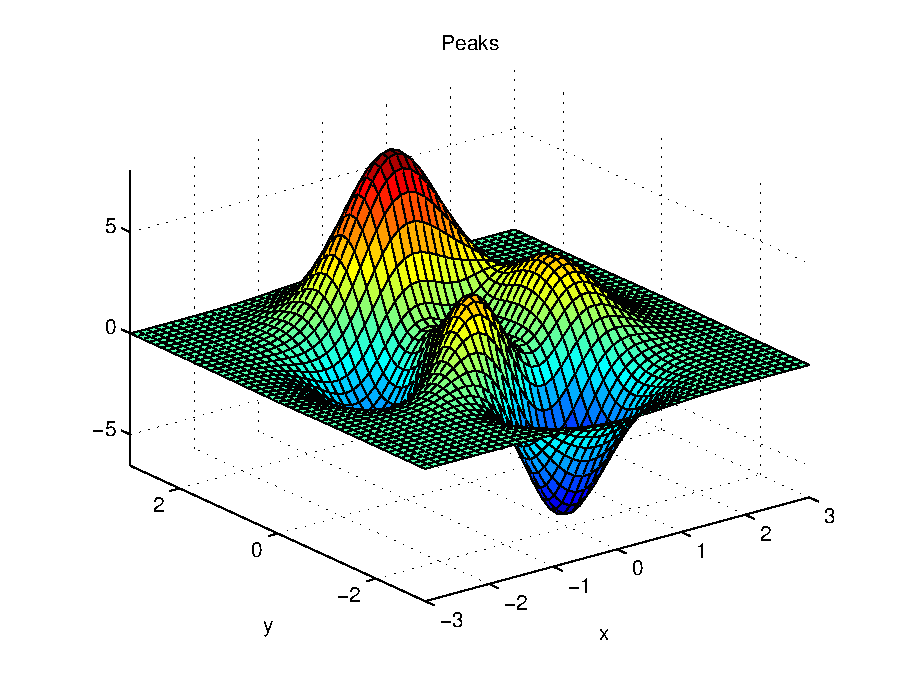
\includegraphics[width=12cm]{mcmthesis-aaa.eps}
    \caption{idk what}
    \label{fig:a}
\end{figure}
\\Reference test \autoref{eq0}

\newpage
\section{Sheet}
\begin{table}[htb]
    \centering
    \caption{My first table}
    \begin{tblr}{
        row{1} = {c},
        cell{2}{1} = {c},
        cell{3}{1} = {c},
        cell{4}{1} = {c},
        cell{5}{1} = {c},
        cell{6}{1} = {c},
        cell{7}{1} = {c},
        hline{1-2,8} = {-}{},
    }
    Variable Name & Meanings \\
    $N$ & Nodes, eg. Ng denotes the set of Goal Nodes \\
    $A$ & Adjacency matrix \\
    $G$ & Relationship Network Model\cite{yang1993tea} \\
    $x$ & The degree of realization of SDGs, as a 1*17 matrix \\
    $\Delta x$ & Perturbations arising, for 1*17 matrix \\
    $c$ & Anti-interference coefficient, related
    \end{tblr}
\end{table}

\bibliography{test}

\end{document} 
